\section{Referencial Teórico}
\label{referencial}

Este capítulo apresenta os fundamentos teóricos que sustentam o desenvolvimento do modelo proposto de legendamento de mudanças em imagens de sensoriamento remoto. O objetivo é situar o trabalho no contexto das pesquisas em detecção de mudanças, aprendizado profundo e geração automática de descrições em linguagem natural, destacando os conceitos, técnicas e arquiteturas que formam a base do \textit{change captioning} em ambiente orbital.

Inicialmente, são discutidos os princípios do monitoramento de mudanças em sensoriamento remoto, enfatizando a evolução de abordagens manuais para métodos automáticos baseados em comparações multitemporais. Em seguida, são revisados os fundamentos de aprendizado profundo em Visão Computacional, com foco em redes convolucionais, arquiteturas siamesas e modelos do tipo \textit{encoder--decoder}, que viabilizaram os avanços recentes em \textit{image captioning}. A partir disso, apresenta-se a adaptação dessas técnicas para o contexto de imagens orbitais e aéreas, no problema de \textit{remote sensing image captioning}, e discute-se o papel dos Transformers e dos mecanismos de atenção na modelagem conjunta de informação visual e textual.

Na sequência, são introduzidos os conceitos específicos de \textit{change captioning} e os principais trabalhos correlatos em sensoriamento remoto, incluindo modelos e conjuntos de dados de referência utilizados na literatura. Por fim, são descritas as métricas de avaliação empregadas na comparação de legendas geradas automaticamente com descrições de referência, as quais serão adotadas na análise experimental deste trabalho. Dessa forma, o referencial teórico busca fornecer uma visão integrada do estado da arte e das lacunas que motivam a proposta aqui desenvolvida.


\subsection{Monitoramento de mudanças em sensoriamento remoto}

O monitoramento de mudanças em áreas geográficas é usado para diversas aplicações, incluindo planejamento urbano, gestão ambiental e resposta a desastres naturais \cite{singh1989,lu2004}. Tradicionalmente, a análise de imagens de sensoriamento remoto multitemporais é feita manualmente por especialistas, que comparam visualmente pares de imagens de diferentes épocas e interpretam elementos como edificações, corpos d’água, áreas de vegetação e superfícies pavimentadas. Além de exigir tempo e mão de obra especializada, esse procedimento é caro e sujeito a diferenças de interpretação entre observadores, o que tem incentivado o desenvolvimento de métodos automáticos, mais objetivos e reprodutíveis para a detecção e descrição dessas mudanças.

\begin{figure}[H]
\centering
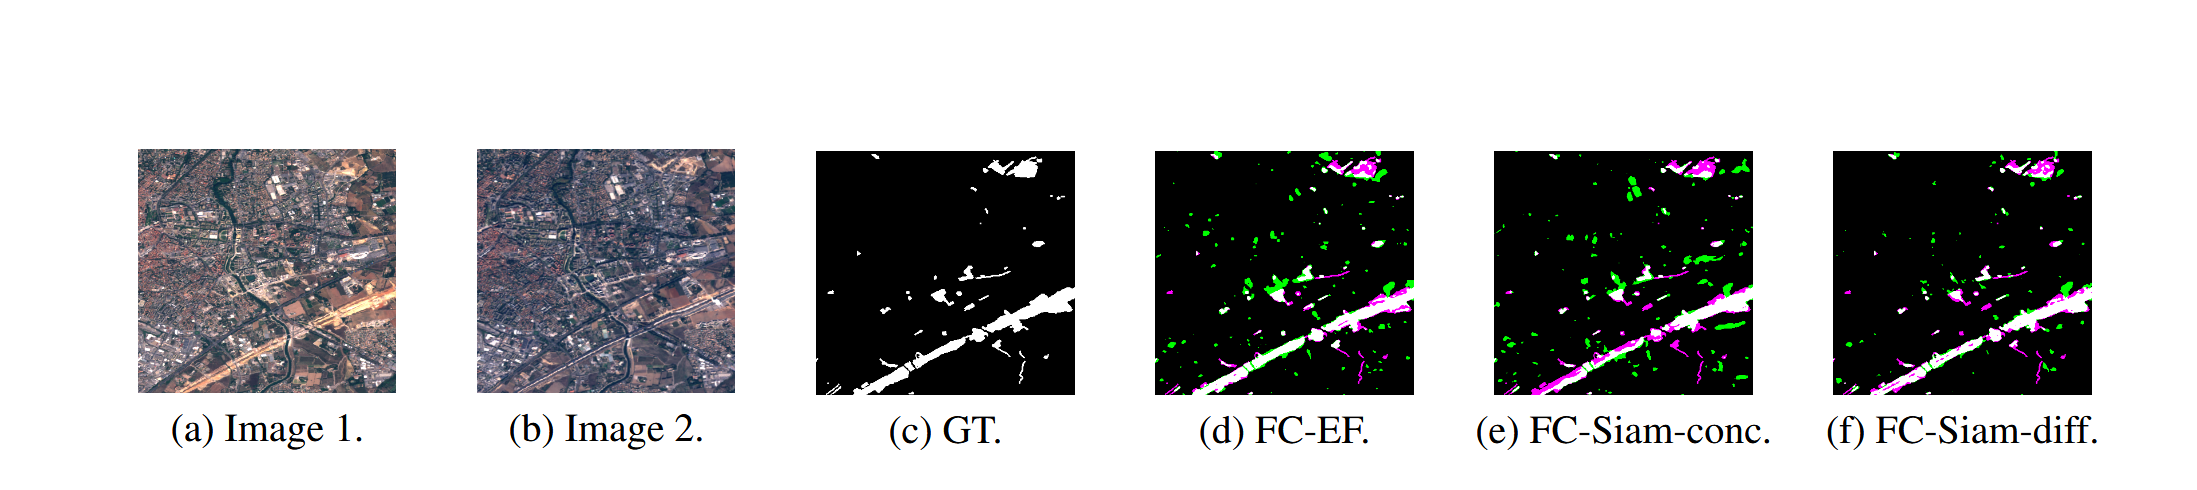
\includegraphics[width=1.1\columnwidth]{figs/fully1.png}
\caption{Exemplo de monitoramento de mudanças. As imagens (a) e (b) representam as datas $t_1$ e $t_2$, e a imagem (c) representa o mapa de mudanças (Ground Truth), onde as alterações são destacadas. Fonte: Daudt et al. \cite{daudt2018}.}
\label{fig-exemplo-cd}
\end{figure}

\subsection{Fundamentos de aprendizado profundo para Visão Computacional}

% O desenvolvimento recente de métodos de detecção e descrição de mudanças em imagens de sensoriamento remoto está diretamente associado ao avanço do aprendizado profundo em Visão Computacional. Em particular, redes neurais convolucionais (CNNs) tornaram-se o principal paradigma para extração de características visuais, devido à sua capacidade de aprender filtros hierárquicos diretamente a partir dos dados, capturando desde padrões locais simples (bordas, texturas) até estruturas de alto nível (objetos e regiões) \cite{lecun2015,krizhevsky2017}.

O desenvolvimento recente de métodos de detecção e descrição de mudanças em imagens de sensoriamento remoto está diretamente associado ao avanço do aprendizado profundo em visão computacional. Redes neurais convolucionais (\textit{Convolutional Neural Networks} — CNNs) tornaram-se o principal paradigma para extração de características visuais, pois aprendem automaticamente filtros hierárquicos diretamente a partir dos dados, capturando desde padrões locais simples (bordas, texturas) até estruturas de nível mais alto (objetos e regiões) \cite{lecun2015,krizhevsky2017}.

% No contexto de comparação entre imagens de épocas diferentes, arquiteturas siamesas passaram a ser amplamente utilizadas. Nesse tipo de arquitetura, duas redes com pesos compartilhados processam, em paralelo, as imagens adquiridas em $t_1$ e $t_2$, produzindo mapas de características que podem ser combinados por operações como diferença, concatenação ou atenção para realçar as regiões em que ocorreram mudanças relevantes \cite{daudt2018}. Essa estratégia reduz o número de parâmetros e incentiva o modelo a aprender representações consistentes entre as duas datas, facilitando a identificação de variações estruturais na cena.

No contexto de comparação entre imagens de épocas diferentes, arquiteturas siamesas passaram a ser amplamente utilizadas. Nesse tipo de arquitetura, duas redes com pesos compartilhados processam, em paralelo, as imagens adquiridas em $t_1$ e $t_2$, produzindo mapas de características que podem ser combinados por operações como diferença, concatenação ou mecanismos de atenção para realçar as regiões em que ocorreram mudanças relevantes \cite{daudt2018}. O compartilhamento de pesos reduz o número de parâmetros do modelo e incentiva o aprendizado de representações consistentes entre as duas datas, o que facilita a identificação de variações estruturais na cena.

Para tarefas que envolvem geração de sequências, como o legendamento automático, é comum empregar arquiteturas do tipo \textit{encoder--decoder}. Nesse arranjo, um \textit{encoder} visual (tipicamente uma CNN, ou uma combinação de CNN e módulos adicionais) mapeia a imagem para um espaço latente, isto é, um vetor de características de dimensão reduzida que sintetiza o conteúdo visual. Em seguida, um \textit{decoder} sequencial produz o texto palavra a palavra, condicionando cada novo token tanto no estado interno do modelo quanto nas características extraídas da imagem. Tradicionalmente, esse \textit{decoder} é implementado com redes recorrentes do tipo LSTM (\textit{Long Short-Term Memory}) ou GRU (\textit{Gated Recurrent Unit}) \cite{vinyals2015}. Essa separação entre a etapa de codificação da imagem e a etapa de geração do texto serviu de base para o desenvolvimento de modelos mais recentes, baseados em Transformers, que substituem as redes recorrentes por blocos de atenção.

\begin{figure}[H]
\centering
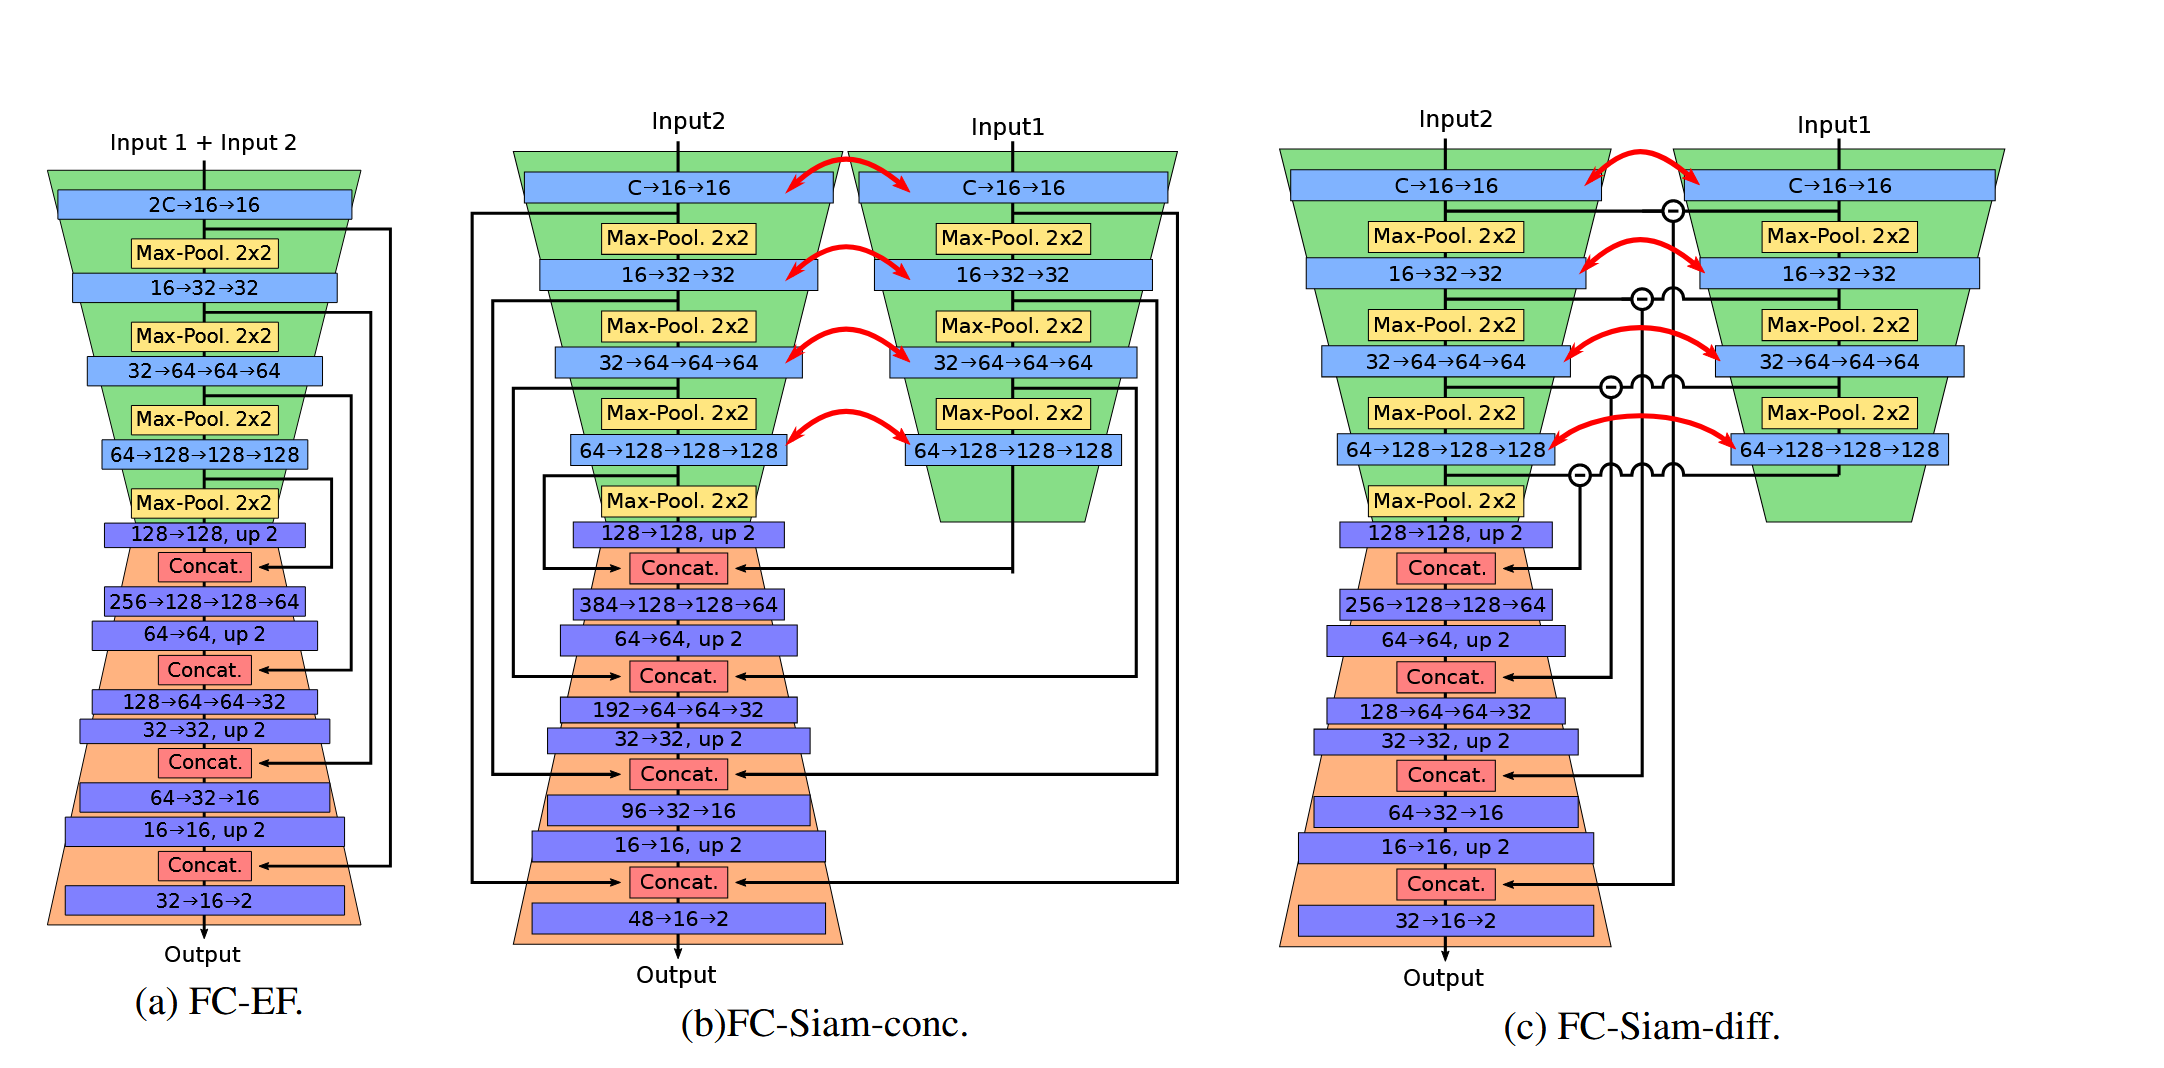
\includegraphics[width=0.5\textwidth]{figs/fully2.png}
\caption{Exemplos de arquiteturas siamesas para detecção de mudanças. O modelo processa duas entradas paralelamente e combina as características para identificar as diferenças. Fonte: Daudt et al. \cite{daudt2018}.}
\label{fig-siamesa}
\end{figure}

% \twocolumn[
% \begin{center}
% \begin{figure}[H] % se usar float H, requer \usepackage{float}
%     \centering
%     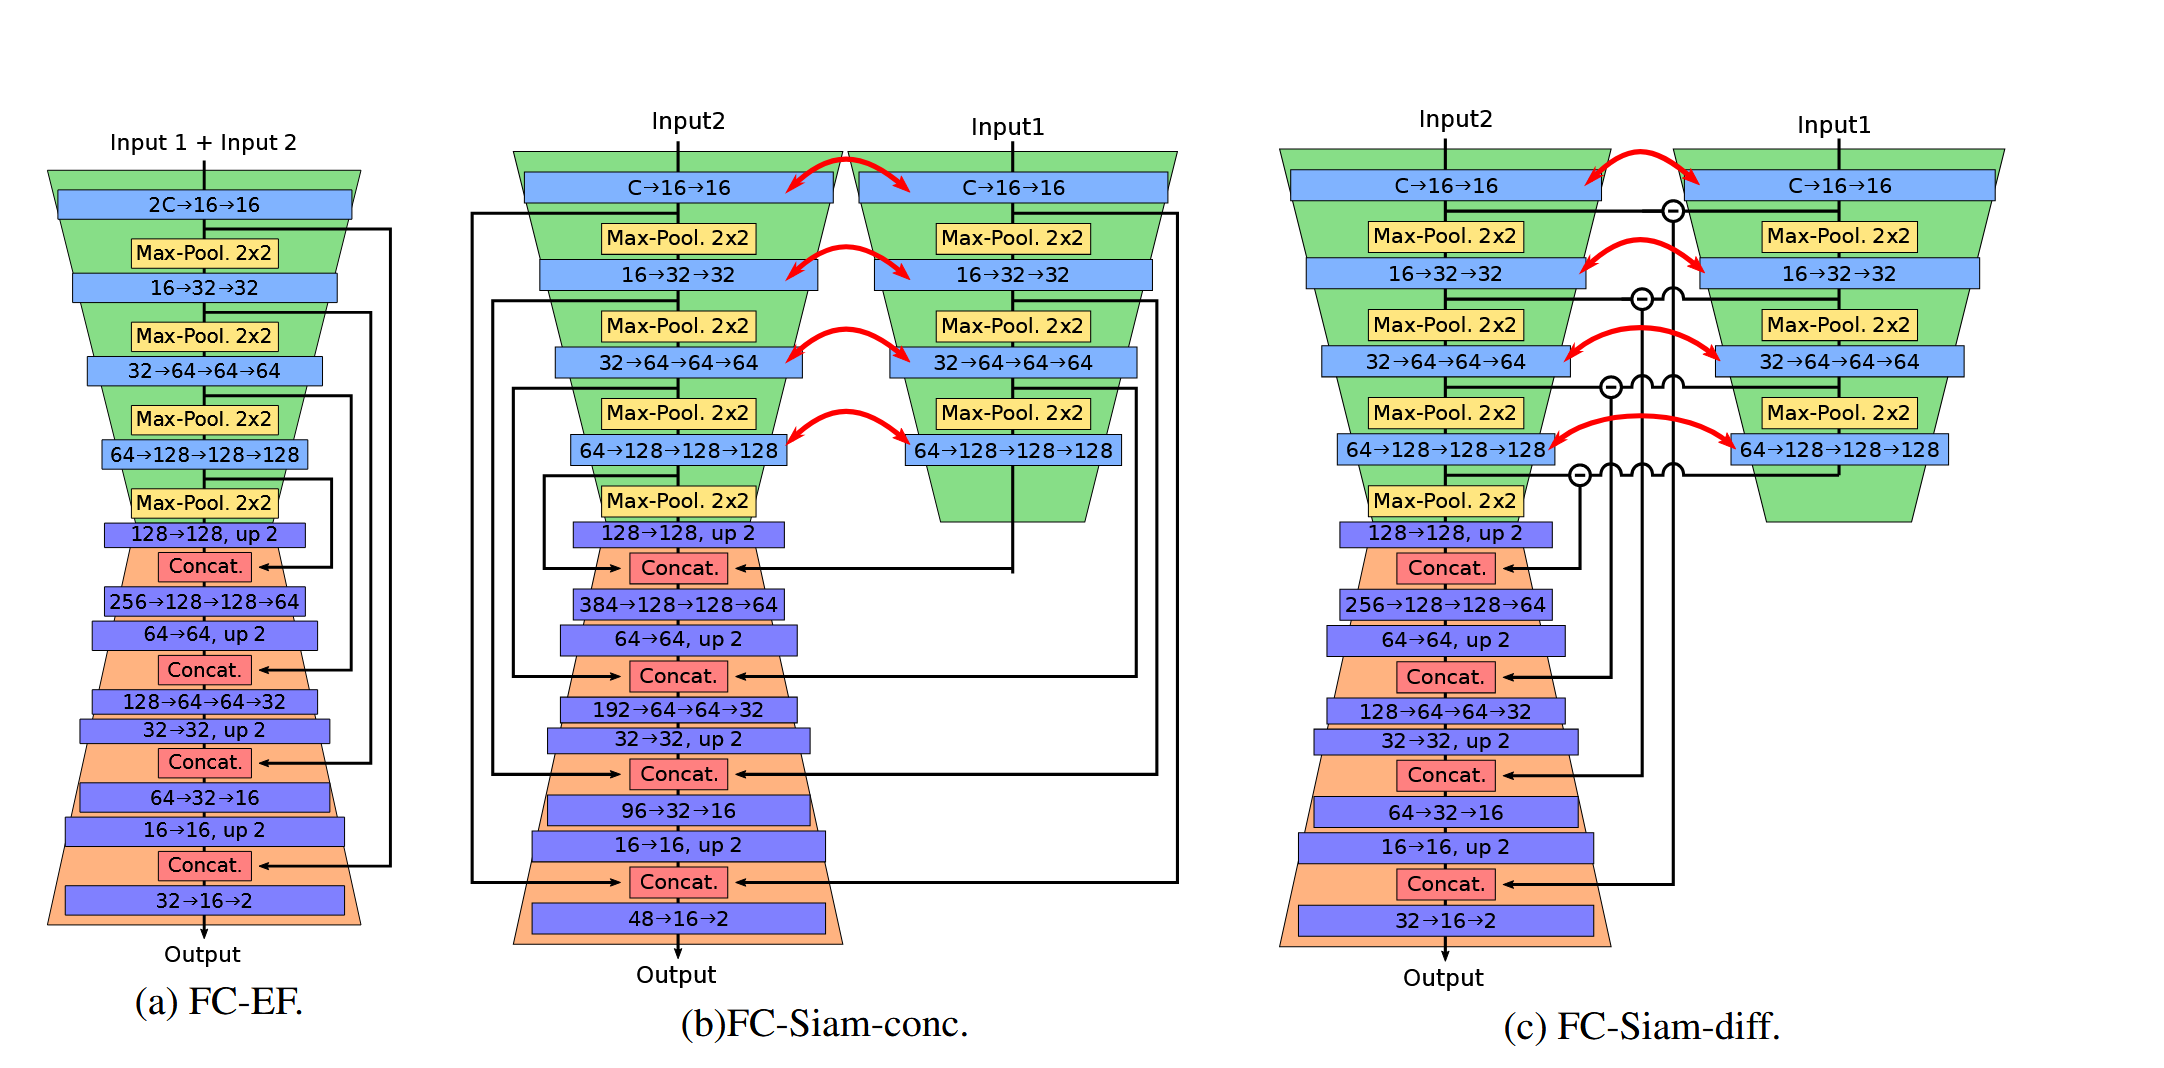
\includegraphics[width=\textwidth]{figs/fully2.png}
% \caption{Exemplos de arquiteturas siamesas para detecção de mudanças. O modelo processa duas entradas paralelamente e combina as características para identificar as diferenças. Fonte: Daudt et al. \cite{daudt2018}.}
% \label{fig-siamesa}
% \end{figure}
% \end{center}


\subsection{Legendamento de imagens (\textit{Image Captioning})}

Na área de visão computacional, o problema de \textit{image captioning} refere-se à tarefa de gerar descrições em linguagem natural a partir de uma única imagem, combinando técnicas de extração de características visuais com modelos de linguagem \cite{vinyals2015,anderson2018}. Nos primeiros modelos baseados em redes neurais profundas, costuma-se empregar uma CNN para extrair um vetor de características da imagem, que é então fornecido a um modelo sequencial (por exemplo, uma rede recorrente do tipo LSTM), responsável por gerar, palavra a palavra, a legenda correspondente.

% Com o avanço das arquiteturas baseadas em aprendizado profundo, especialmente modelos do tipo \textit{encoder--decoder} com mecanismos de atenção, tornou-se possível produzir descrições mais ricas e coerentes, aproximando-se da forma como humanos descrevem cenas visuais \cite{lecun2015}. O mecanismo de atenção permite que o modelo foque dinamicamente em diferentes regiões da imagem ao longo da geração da frase, capturando melhor relações espaciais e detalhes semânticos relevantes.

Com a evolução das arquiteturas de aprendizado profundo, especialmente modelos do tipo \textit{encoder--decoder} com mecanismos de atenção, passou a ser possível produzir descrições mais detalhadas e consistentes \cite{anderson2018}. O mecanismo de atenção permite que o modelo foque dinamicamente em diferentes regiões da imagem ao longo da geração da frase, capturando relações espaciais e detalhes semânticos relevantes.

\subsection{Legendamento de imagens de sensoriamento remoto (\textit{Remote Sensing Image Captioning})}


No contexto de sensoriamento remoto, esses avanços deram origem ao problema de \textit{remote sensing image captioning}, em que as técnicas de legendamento são adaptadas para imagens orbitais e aéreas. Nesse cenário, é necessário lidar com características específicas, como a visão em ``vista de topo'' (\textit{top view}), a presença de objetos em diferentes escalas e a grande variabilidade de padrões espaciais em áreas urbanas, rurais e naturais.

Os métodos de \textit{remote sensing image captioning} buscam não apenas identificar objetos presentes na cena (como edificações, vias, áreas de vegetação e corpos d'água), mas também descrever suas relações espaciais e funcionais, tornando os produtos de sensoriamento remoto mais acessíveis para usuários não especialistas. Trabalhos recentes têm explorado arquiteturas baseadas em Transformers para o legendamento de imagens de sensoriamento remoto em uma única data, evidenciando o potencial desses modelos para capturar dependências de longo alcance na imagem e no texto \cite{nanal2023}.

\begin{figure}[H]
\centering
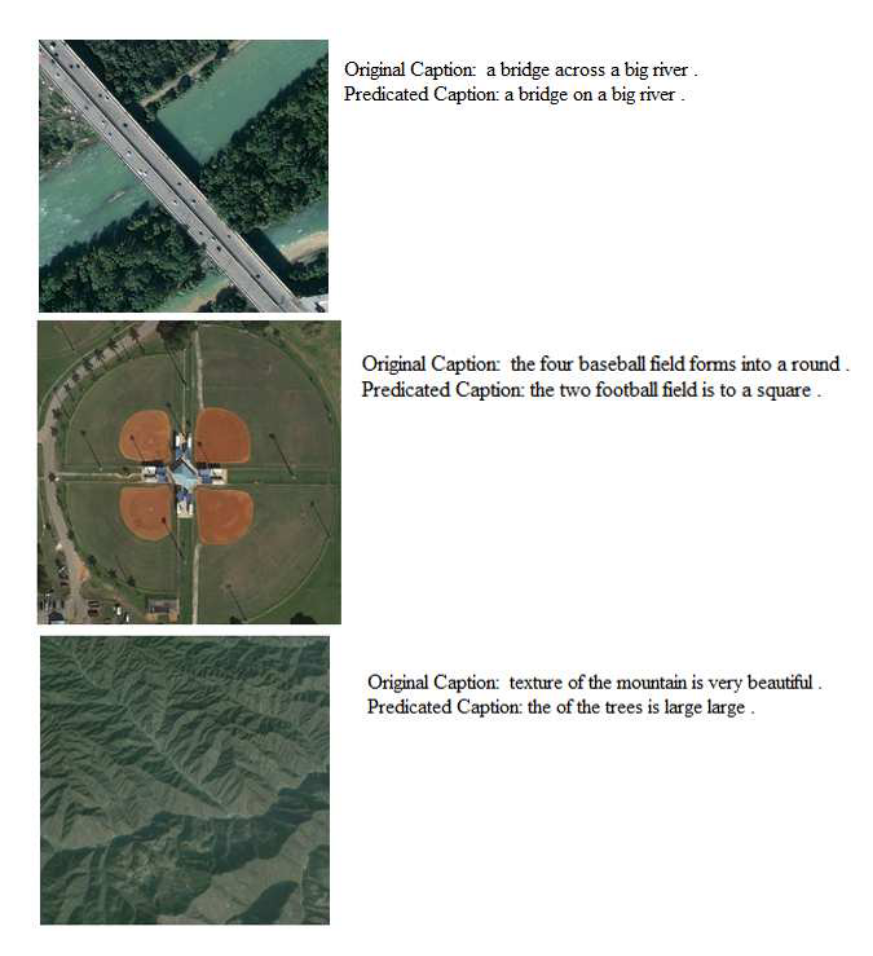
\includegraphics[width=0.9\columnwidth]{figs/rsic1.png}
\caption{Exemplos de legendamento de imagens de sensoriamento remoto (\textit{Remote Sensing Image Captioning}). O modelo descreve o conteúdo estático da cena, como pontes e campos esportivos. Fonte: Nanal e Hajiarbabi \cite{nanal2023}.}
\label{fig-exemplo-rsic}
\end{figure}

\subsection{Transformers e mecanismos de atenção}

Os Transformers introduziram uma forma distinta de modelar dependências de longo alcance em sequências, substituindo as conexões recorrentes tradicionais por mecanismos de autoatenção \cite{vaswani2017}. De maneira simplificada, a autoatenção permite que cada elemento de uma sequência (por exemplo, uma palavra ou um vetor de características visuais) estabeleça relações diretas com todos os demais, atribuindo pesos de atenção aprendidos durante o treinamento a cada uma dessas relações. Com isso, o modelo consegue destacar automaticamente os elementos mais relevantes do contexto, o que favorece a captura de dependências globais e permite uma paralelização mais eficiente do que em arquiteturas recorrentes.

Em legendamento de imagens, os Transformers podem atuar tanto no módulo visual quanto no módulo textual. No decodificador, a atenção mascarada sobre a sequência de palavras garante que a predição de cada token considere apenas o histórico já gerado, enquanto a atenção cruzada (\textit{cross-attention}) conecta o texto às representações visuais da imagem ou de regiões específicas. Em aplicações de sensoriamento remoto, esse mecanismo é particularmente útil para relacionar descrições textuais a estruturas espaciais complexas presentes na cena.

No caso do \textit{change captioning}, o uso de Transformers abre a possibilidade de explorar, de forma mais rica, as interações entre as representações das imagens em $t_1$ e $t_2$. Modelos como o RSICCformer empregam codificadores de dois ramos (\textit{dual-branch encoders}), nos quais cada ramo processa uma das datas, e camadas de atenção são responsáveis por estabelecer relações entre as duas representações ao longo da cena \cite{liu2022}. Essa estratégia permite que o modelo identifique não apenas a presença ou ausência de objetos, mas também como sua configuração espacial evolui no tempo, o que é fundamental para gerar descrições de mudança coerentes e informativas.

\subsection{Legendamento de mudança (\textit{Change Captioning})}

Mais recentemente, surge o paradigma de \textit{change captioning} (legendamento de mudança), que estende o problema de \textit{captioning} para o caso de imagens multitemporais. Em vez de descrever apenas o conteúdo de uma única imagem, o objetivo é gerar frases que descrevam explicitamente as mudanças observadas entre duas aquisições de uma mesma área ao longo do tempo \cite{park2019,liu2022}. 

Nesse contexto, combinam-se técnicas de Visão Computacional e Processamento de Linguagem Natural para produzir descrições como ``novos edifícios foram construídos na região central'' ou ``áreas de vegetação foram substituídas por pavimentação''. Em contraste, métodos tradicionais de detecção de mudanças em sensoriamento remoto, como redes siamesas totalmente convolucionais, tipicamente produzem apenas mapas binários ou categóricos indicando regiões alteradas \cite{daudt2018}. O \textit{change captioning}, por sua vez, fornece um resumo textual de alto nível, mais facilmente interpretável por usuários finais e potencialmente integrável a sistemas de apoio à decisão.

\begin{figure}[H]
\centering
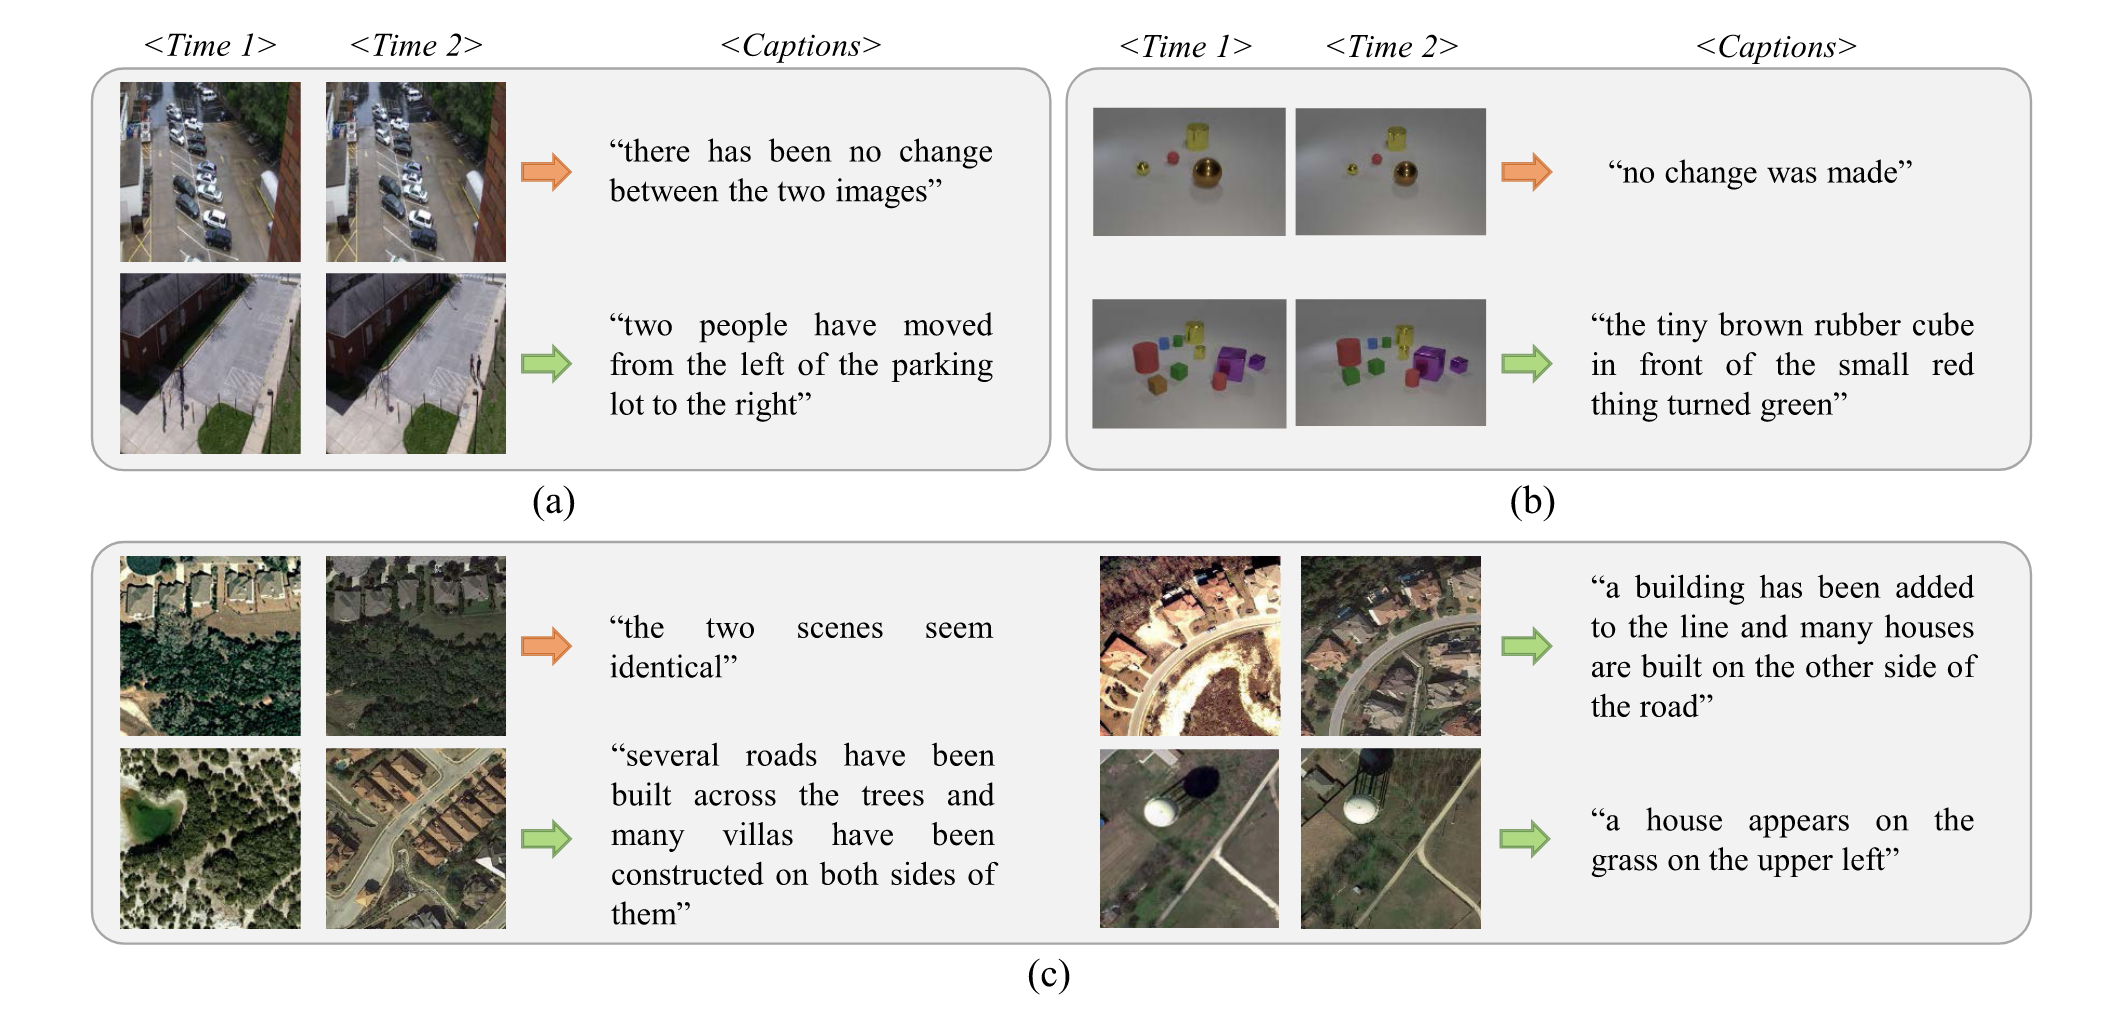
\includegraphics[width=1.0\columnwidth]{figs/chg2cap1.png} 
\caption{Exemplos de legendamento de mudança em diferentes domínios: (a) imagens naturais de vigilância; (b) imagens sintéticas com mudanças de ponto de vista; e (c) imagens de sensoriamento remoto do dataset LEVIR-CC. Fonte: Adaptado de Chang e Ghamisi \cite{chang2023}.}
\label{fig-chg2cap1}
\end{figure}

\subsection{Trabalhos correlatos em \textit{change captioning} para sensoriamento remoto}

Nos últimos anos, diversos modelos específicos para \textit{change captioning} em sensoriamento remoto têm sido propostos, combinando extratores visuais profundos com \textit{decoders} recorrentes ou baseados em Transformers. Entre esses trabalhos, destaca-se o \textit{Chg2Cap}, que utiliza uma arquitetura siamesa de CNNs para extrair características das imagens bitemporais e módulos de atenção para localizar regiões de mudança e gerar descrições textuais correspondentes \cite{chang2023}. Esse modelo explora explicitamente a diferença entre as duas datas, buscando concentrar a geração de texto nas áreas em que mudanças relevantes ocorreram.

Outro marco importante é o conjunto de dados \textit{LEVIR-CC}, construído a partir de uma base de detecção de mudanças de edificações em imagens de alta resolução. Esse conjunto de dados associa pares de imagens bitemporais a legendas que descrevem as mudanças observadas, tornando-se um dos principais referenciais para treinamento e avaliação de modelos de \textit{change captioning} em sensoriamento remoto \cite{liu2022}. No mesmo trabalho em que o \textit{LEVIR-CC} é apresentado, os autores propõem o modelo \textit{RSICCformer}, que combina um extrator de características baseado em CNN, um codificador Transformer de dois ramos (\textit{dual-branch encoder}) e um decodificador de legendas para capturar múltiplas mudanças de interesse em pares de imagens, obtendo ganhos significativos em métricas como BLEU-4 e CIDEr-D em relação a abordagens anteriores \cite{liu2022}.

Complementarmente, o trabalho de Hoxha \cite{hoxha2022} formaliza o \textit{change captioning} como um novo paradigma para análise de imagens multitemporais de sensoriamento remoto, discutindo como descrições textuais de mudança podem enriquecer e complementar os mapas de mudança tradicionais.

Além disso, modelos baseados em Transformer aplicados ao \textit{remote sensing image captioning} em uma única data também têm mostrado bom desempenho, reforçando o potencial dessas arquiteturas para tarefas de descrição automática em sensoriamento remoto \cite{nanal2023}. O modelo proposto neste trabalho se insere nesse contexto, buscando explorar de forma mais eficiente as interações entre as representações das imagens em $t_1$ e $t_2$ para gerar descrições de mudança mais precisas e informativas.

\begin{figure}[H]
\centering
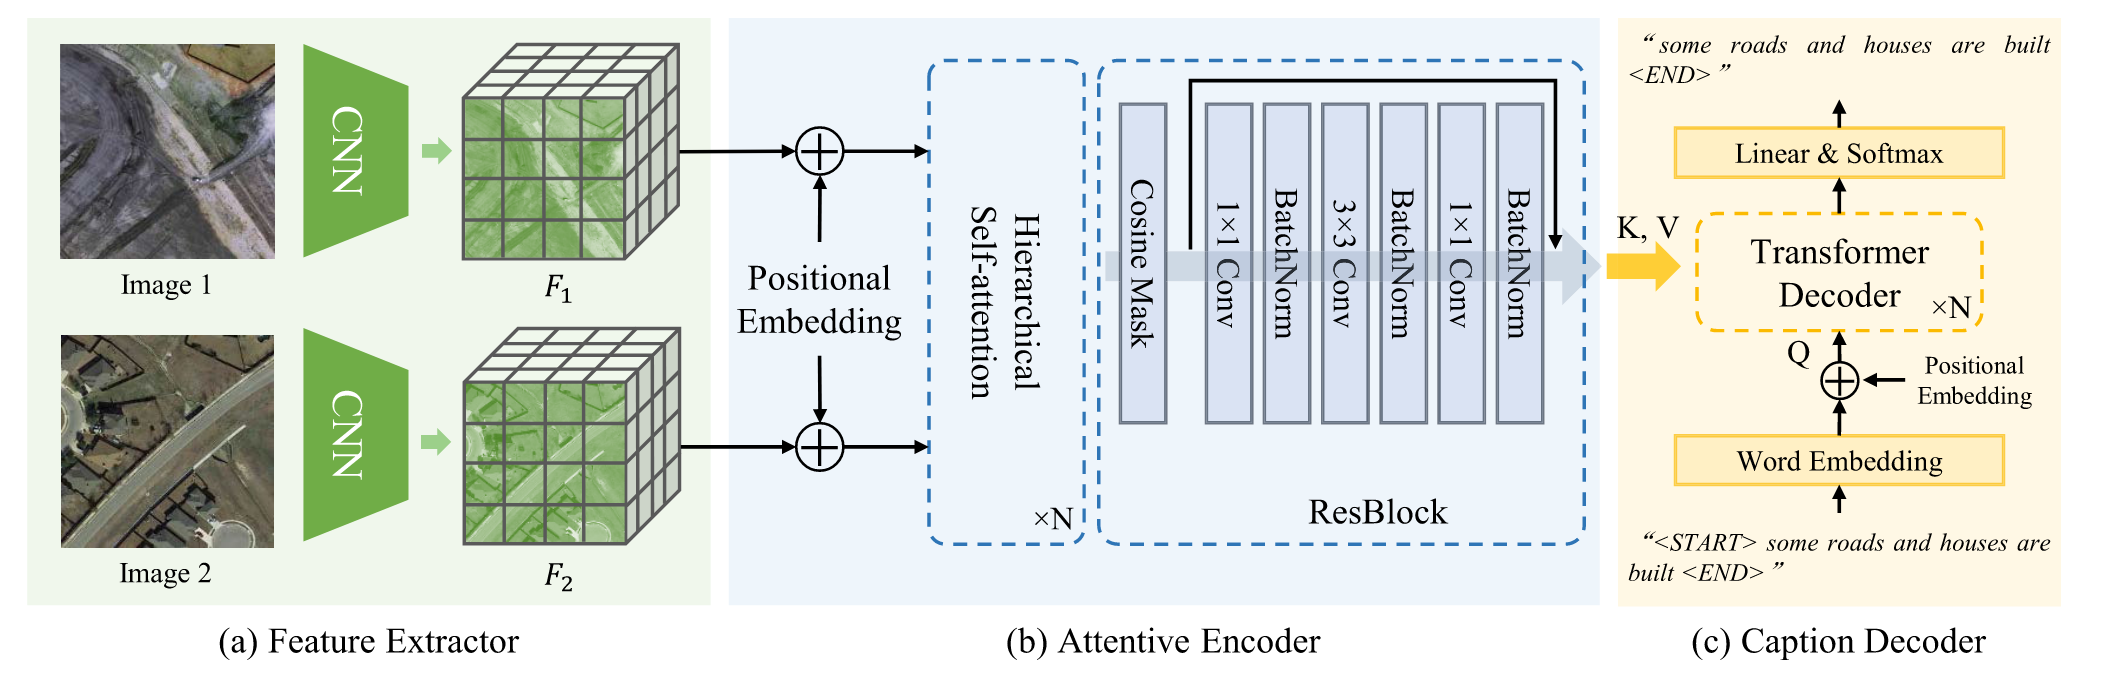
\includegraphics[width=1.0\columnwidth]{figs/chg2cap2.png}
\caption{Estrutura geral do modelo Chg2Cap. O modelo é composto por (a) um extrator de características baseado em CNN, (b) um codificador atento com blocos de autoatenção hierárquica e (c) um decodificador de legendas. Fonte: Chang e Ghamisi \cite{chang2023}.}
\label{fig-chg2cap2}
\end{figure}

% \usepackage{sttools}  % ou cuted

% \begin{strip}
% \begin{center}
% 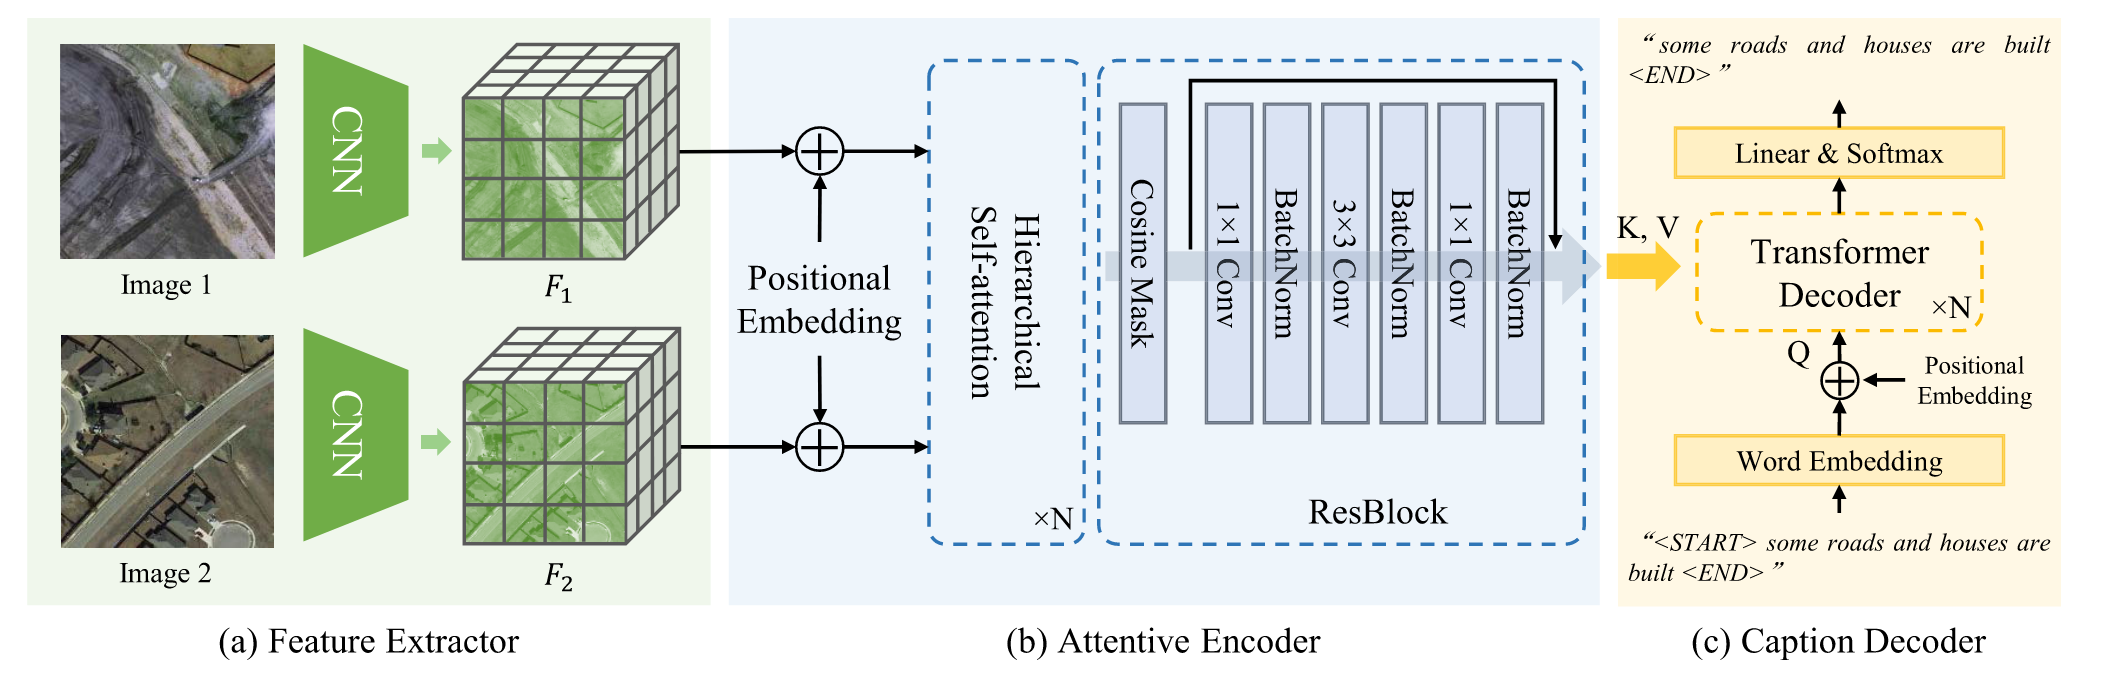
\includegraphics[width=\textwidth]{figs/chg2cap2.png}
% \captionof{figure}{Estrutura geral do modelo Chg2Cap. O modelo é composto por (a) um extrator de características baseado em CNN, (b) um codificador atento com blocos de autoatenção hierárquica e (c) um decodificador de legendas. Fonte: Chang e Ghamisi \cite{chang2023}.}
% \label{fig-chg2cap2}
% \end{center}
% \end{strip}

\subsection{Métricas de avaliação para legendamento automático}

A avaliação de modelos de legendamento automático é, em grande parte, baseada na comparação entre as frases geradas pelo modelo e um conjunto de legendas de referência anotadas manualmente. Para esse fim, diferentes métricas têm sido propostas, cada uma enfatizando aspectos específicos de similaridade textual, como coincidência de n-gramas, correspondência semântica ou estrutura de dependências.

Entre as métricas automáticas mais utilizadas está o BLEU (\textit{Bilingual Evaluation Understudy}), que calcula a precisão de n-gramas entre a legenda gerada e as legendas de referência, penalizando legendas excessivamente curtas \cite{papineni2002}. O METEOR, por sua vez, combina informação de precisão e cobertura (\textit{recall}), incorporando também variações morfológicas e sinônimos, o que o torna mais sensível à qualidade semântica das sentenças \cite{banerjee2005}. Outras métricas relevantes incluem o ROUGE-L, baseado em subsequências comuns mais longas, e o CIDEr, que pondera n-gramas pela sua frequência no conjunto de legendas, enfatizando termos mais específicos do domínio \cite{vedantam2015}.

Em trabalhos recentes de \textit{image captioning} e \textit{change captioning} em sensoriamento remoto, é comum reportar um conjunto dessas métricas em conjunto, de forma a obter uma visão mais abrangente do desempenho dos modelos. Além das medidas textuais, alguns estudos também consideram métricas derivadas de tarefas relacionadas, como a qualidade de mapas de mudança (por exemplo, IoU e F1), quando o modelo produz simultaneamente saídas visuais e textuais. Neste trabalho, as métricas selecionadas para avaliação são aquelas mais consolidadas na literatura de legendamento automático, permitindo a comparação com abordagens previamente publicadas e com o estado da arte na área.
